\documentclass[a4,11pt]{aleph-notas}

% -- Paquetes adicionales
\usepackage{enumitem}
\usepackage{aleph-comandos}


% -- Datos 
\institucion{Escuela de Ciencias Físicas y Matemática}
\carrera{Ciencia de DAtos}
\asignatura{Álgebra lineal}
\tema{Clase invertida no. 1: Independencia Lineal}
\autor[A. Merino]{Andrés Merino}
\fecha{Semestre 2024-1}

\logouno[0.14\textwidth]{Logos/logoPUCE_04_ac}
\definecolor{colortext}{HTML}{0030A1}
\definecolor{colordef}{HTML}{0030A1}
\fuente{montserrat}

% -- Comandos adicionales
\begin{document}

\encabezado

\vspace*{-10mm}
\section*{Introducción}

\begin{itemize}
    \item \textbf{Tema:} Independencia Lineal
    \item \textbf{Resultado de Aprendizaje:} Determina si un conjunto de vectores el linealmente independiente.
\end{itemize}

\section*{Lección en casa}

\subsection*{Actividades}

\begin{enumerate}[leftmargin=*]
    \item Interactuar con ChatGPT mediante los siguientes \textit{prompts}, leyendo detenidamente el \textit{prompt} y su respuesta:
    \begin{enumerate}[label=\textit{Prompt \arabic*.},leftmargin=2.1cm]
        \item Vas a ser mi profesor de la asignatura de Álgebra Lineal, te iré dando indicaciones y me irás explicando de manera formal y luego de manera intuitiva los conceptos. Vas a tener mucho cuidado al escribir la parte matemática para que se visualice bien. Sé amable. ¿Entendido?
        \item Dado un espacio vectorial E y un conjunto de vectores, ¿qué significa que sea linealmente independientes?
        \item ¿Cómo se determina si un conjunto de vectores es linealmente independiente? Explícame paso a paso. No me des un ejemplo aún.
        \item Explícame cómo se determina que estos dos vectores son linealmente independientes: (1,2), (2,1). 
        \item Explícame cómo se determina que estos dos vectores no son linealmente independientes: (1,2), (2,4). 
        \item Ahora, dame un ejemplo con vectores de R3.
        \item Ahora dame un ejemplo en matrices de 2 por 2.
        \item Ahora, dame un ejemplo en polinomios de grado 2.
        \item Plantéame dos ejercicios donde debo determinar si un conjunto de vectores es linealmente independiente o no.
        \item Evalúame para determinar si he comprendido. Escríbeme una pregunta de opción múltiple y te daré la respuesta, luego me darás retroalimentación.
    \end{enumerate}
    \item Continuar la interacción hasta que te sientas preparado en el entendimiento del concepto.
    \item Copiar el enlace del chat como evidencia del proceso (ver Anexo).
    \item En caso de tener dudas sobre el tema, interactúa con tus compañeros de clase para solventarlas.
    \item Realiza el cuestionario del aula virtual.
\end{enumerate}

\section*{Anexo}

\subsection*{¿Cómo obtener el enlace de una conversación con ChatGPT?}

Seguir los siguientes pasos:
\begin{enumerate}
    \item Dar clic en los tres puntos a lado del nombre de la conversación.
    \item Seleccionar «Compartir».
    \begin{center}
        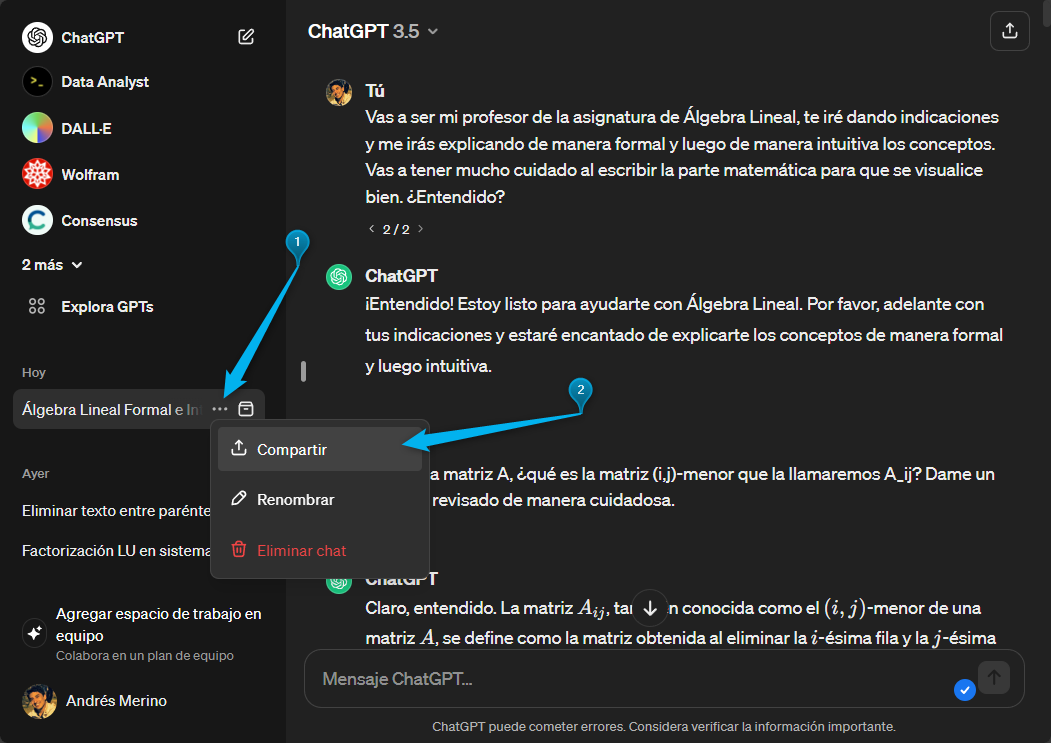
\includegraphics[width=0.85\linewidth]{fig01.png}
    \end{center}
    \item En la nueva ventana, dar clic en los tres puntos. 
    \item Seleccionar «Compartir tu nombre».
    \item Dar clic en «Compartir enlace».

    \begin{center}
        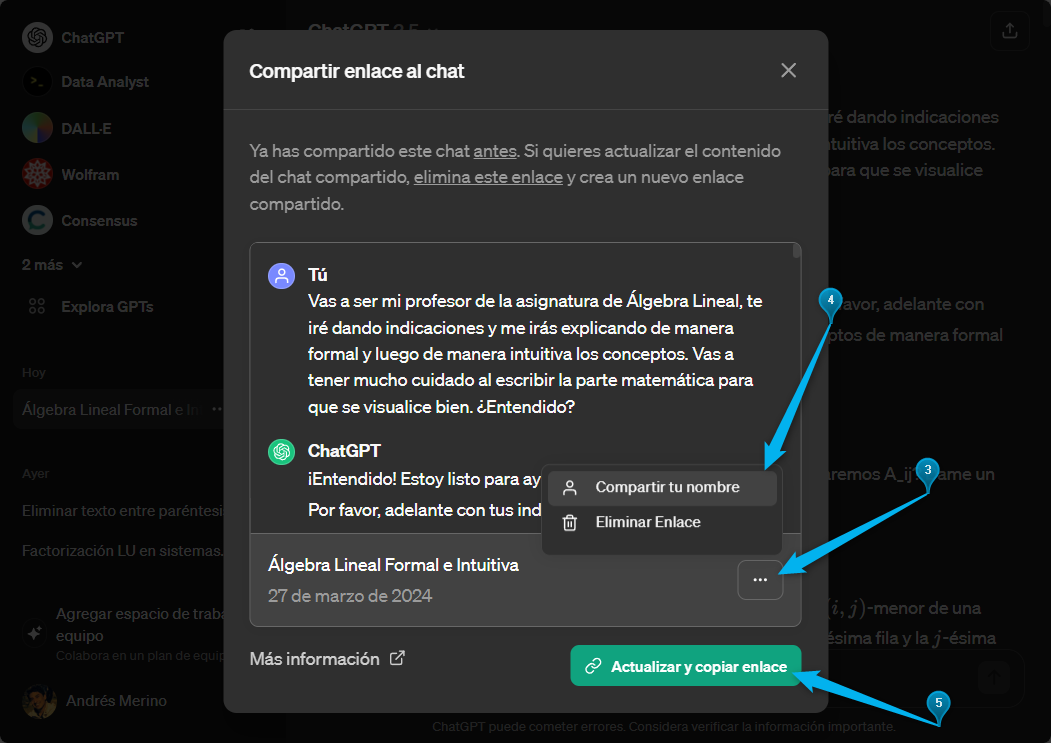
\includegraphics[width=0.85\linewidth]{fig02.png}
    \end{center}
\end{enumerate}


\end{document}